% \documentclass[12pt,a4paper,oneside]{book}
\documentclass[12pt,a4paper,twoside]{book} % zamienilem z twoside na oneside zeby na kazdej stronie bylo

\usepackage{pre}

\title
    {
    \vspace{-2.5cm}
        {
\includegraphics[width=.215\textwidth]{figs/PWrLogo.eps}} \par \vspace{1ex} \large{POLITECHNIKA WROCŁAWSKA} 
	\par \vspace{1ex}
	{\scshape\large Wydział Podstawowych Problemów Techniki\par}
	\vspace{2cm}
    {Praca inżynierska\par}  % Pozostaw inżynierska albo magisterska.
    \vspace{2cm}
	{\Large{\bf Rozwój mobilnej aplikacji do rozpoznawania języka migowego z wykorzystaniem transformerów}\par}
    {Development of mobile application for sign language recognition using transformers}
    }
    
\author
    {
    \vspace{1cm}
    Autor: Maciej Grzesik asda asds\\
    Opiekun: Prof. uczelni dr hab. Sebastian Kraszewski 
    }
\date{\vfill Wrocław~2024}

%%% BEGINNING OF THE THESIS %%%

\begin{document}

\maketitle

\afterpage{\blankpage}\clearpage

\begin{flushright}
    \thispagestyle{empty}
    \vspace*{\fill}
    {
        \em Moim \dots
    }
\end{flushright}

\afterpage{\blankpage}\clearpage

{
  \hypersetup{linkcolor=black}
  \tableofcontents
}

%%%%%%%%%%%%%%%%%%%%%%%%%%%%%%%%%%%%%%
% IT IS GOOD TO WRITE EACH SENTENCE IN A SEPARATE LINE,
% BECAUSE THIS HELPS FIND A PARTICULAR SENTENCE BY SIMPLY
% EYE-SCANNING THE LEFT EDGE OF THE .TEX FILE.
% IT IS ALSO EASY TO SWITCH ON/OFF A PARTICULAR SENTENCE BY COMMENTING IT OUT.
% BESIDES, IN REAL-TIME DISCUSSIONS ONE CAN REFER TO 
% A PARTICULAR SENTENCE BY A SPECIFIC LINE OF THE .TEX FILE.
%%%%%%%%%%%%%%%%%%%%%%%%%%%%%%%%%%%%%%

\chapter{Wprowadzenie}\label{ch:intro}

\section{Motywacja}

Wykluczenie społeczne osób głuchoniemych stanowi poważny problem w społeczeństwie, wynikający z braku mozliwości komunikacji werbalnej w sferze publicznej. 
Uszkodzenie słuchu, szczególnie w życiu codziennym, powoduje trudności w~komunikacji z otoczeniem, które opiera się na konwencjonalnej mowie.
Rodzi to problem z mozliwością partycypacji w prostych aktywnościach poczynając od uczestniczenia w zyciu społecznym do m.in. jakości otrzymywanych usług medycznych.

Nalezy zaznaczyć, iz znajomość języka migowego wsród ludzi zdrowych ogranicza się do sytuacji w których osoby im bliskie są dotknięte problemem uszkodzonego słuchu.  
Język ten, będący podstawową formą komunikacji dla osób głuchoniemych nie jest szeroko nauczany a jego znajomość często wymaga zaangazowania się w dodatkowe kursy tudziez szkolenia, nierzadko płatne.

Na podstawie badań Pauliny Malczewskiej wynika, że aż 90\% ankietowanych głuchoniemych doświadcza alienacji oraz dyskryminacji ze strony słyszących \cite{malczewska2011}.
Zjawiska te niezaprzeczalnie przyczyniają się do przewlekłego obnizenia nastroju, lęku przed byciem postrzeganym przez społeczeństwo oraz ogólnym spadkiem poczucia własnej wartości i samooceny. 
Te aspekty stawiają solidny grunt pod rozwój chorób psychicznych tj. depresja, epizody nastroju depresyjnego, zaburzenia adaptacyjne czy fobii społecznej co potwierdzają poszczególne wytyczne diagnostyczne zawarte w DSM-5 \cite{american2013diagnostic}.

Istotnym jest zaadresowanie tego problemu za pomocą aplikacji wspierającej osoby głuchonieme.
Nie tylko ułatwi to komunikację, ale także przyczyni się do zwiększenia inkluzywności społecznej, zapewniając równe szanse i redukując poziom dyskryminacji.


\section{Cel}\label{sec:aim}

Głównym celem pracy jest stworzenie algorytmu opertego na transofrmerach czyli na architekturze głębokiego uczenia maszynowego, którego zadaniem będzie klasyfikacja znaków języka migowego.
Istotnym jest zasięgnięcie do rozwiązań opartych na uczeniu maszynowym gdyz rozwiązania oparte na algorytmice nie sprawdzają się w przypadkach dotyczących widzenia komputerowego, które jest znaczącym elementem tej pracy. [elaborate on this]
Umozliwi to tłumaczenie języka migowego na tekst w czasie rzeczywistym, co ułatwi komunikację osobom głuchoniemym. 

Sam algorytm zaimplementowany zostanie w aplikacji mobilnej docelowo dedykowanej na smartfony z systemem oparacyjnym Android oraz iOS. Mozliwe jest to dzięki wykorzystaniu środowiska Flutter, które pozwala na tworzenie oprogramowania opartego o język Dart, a następnie na kompilowanie kodu przy wykorzystaniu natywnych narzędzi kompilacyjnych (Android Studio dla systemu Android; Xcode dla systemu iOS).

\section{Zakres}\label{sec:scope}

W ramach pracy inżynierskiej zaprojektowany zostanie przyjazny interfejs użytkownika, który umożliwi proste korzystanie z aplikacji zarówno przez osoby głuche, jak i słyszące.
Wykorzystanie środowiska Flutter pozwoli na implementacje interaktywnego interfejsu użytkownika przy wykorzystaniu wbudowanych funkcjonalności.
Dodatkowo zostanie wyeliminowana potrzeba pisania kodu w natywnym dla danego środowiska języku, co zapewnia aplikacji możliwość działania na różnych mobilnych systemach operacyjnych.

Zostanie również przeprowadzona implementacja oraz trening modelu.
W tym etapie projektu zostaną zastosowane odpowiednie algorytmy, które umożliwią skuteczne uczenie modelu na podstawie zebranych danych dotyczących gestów języka migowego.
Proces uczenia będzie obejmował zarówno fazę wstępną, w której model będzie dostosowywany do charakterystyki danych, jak i fazę walidacji, w której oceni się jego dokładność i zdolność do generalizacji gestów języka migowego.
Istotynm jest również przeprowadzenie testów funkcjonalności modelu w warunkach rzeczywistych aby potwierdzić jego poprawne działanie lub wprowadzanie ewentualnych poprawek.  

\chapter{Teoria}

Transformery to zaawansowane modele uczenia maszynowego, szeroko stosowane w przetwarzaniu języka naturalnego, wizji komputerowej, ale~także w audio i~przetwarzaniu multimedialnym. \\ 
W odróżnieniu od poprzednio stosowanych modeli uczenia maszynowego opierających się na podejściu rekurencyjnym i mechanizmie uwagi, naukowcy pracujący dla firmy Google zaproponowali rozwiązanie wykorzystujące jedynie mechanizm uwagi. Skutkiem tego podejścia jest znaczne przyspieszenie czasu uczenia modelu przy zachowaniu wysokiej precyzji \cite{vaswani2023attentionneed}.
\section{Zasada działania}
Działanie transformera opiera się na warstwie kodującej oraz na warstwie dekodującej.
Zadaniem warstwy kodującej jest zakodowanie argumentów wejściowych (np. tekstu, obrazów) do postaci numerycznej. Warstwa dekodująca, wykorzystuje przekazane z warstwy kodującej zakodowane informacje do przetworzenia ich na wartości wyjściowe (np. do tekstu czy wideo). \\
Istotnym elementem, który różnicuje transformery od rekurencyjnych modeli uczenia maszynowego jest mechanizm uwagi. W tradycyjnych modelach rekurencyjnych sieci neuronowych (RNN) dane przetwarzane są sekwencyjnie tzn., że są analizowane krok po kroku (patrz \ref{fig:rnn_schema}) \cite{mamczur2020} co skutkuje ograniczeniami m.in. w równoległości przetwarzaniu danych.

\begin{figure}[h]
    \centering
	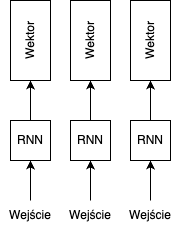
\includegraphics[scale=0.75]{figs/rnn.png}
	\caption{Przepływ informacji wejściowych w rekurencyjnych sieciach neuronowych}
	\label{fig:rnn_schema}
\end{figure}

\pagebreak

Rozwiązania inżynieryjne wykorzystane w transformerach pozwalają modelom na przetwarzanie wszystkich elementów sekwencji jednocześnie (patrz \ref{fig:transformer_schema}).

\begin{figure}[h]
    \centering
	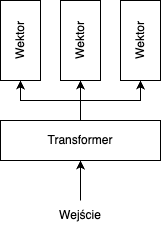
\includegraphics[scale=0.75]{figs/transformer.png}
	\caption{Przepływ informacji wejściowych w transformerach}
	\label{fig:transformer_schema}
\end{figure}

W praktyce oznacza to, że uczenie transformerów przebiega w określonej stałej ilości $O(1)$ sekwencyjnie wykonywanych operacji, modele RNN wymagają natomiast $O(n)$ sekwencyjnie wykonywanych operacji co sprawia, że są mniej wydajne przy dłuższych sekwencjach.

\pagebreak

\section{Architektura}

Zanim dane przetwarzane przez transformer zostaną przekazane do kodera muszą zostać wstępnie przetworzone. Proces ten można podzielić na dwa kroki:
\begin{itemize}
    \item Input Embedding polega na zamienieniu danych wejściowych na przystępne dla obliczeń komputerowych wektory.
    \item Positional Encoding składa się z wektorów, których zadaniem jest nadanie kontekstu na podstawie pozycji danych w sekwencji. Jest to istotne, gdyż z~punktu widzenia maszyny nie jest wstanie odróżnić ona informacji użytych w różnym znaczeniu. 
\end{itemize}
Sam koder składa się z dwóch elementów:
\begin{itemize}
    \item Multi-Head Attention polega na obliczeniu wektora uwagi dla poszczególnych informacji przekazanych do tej warstwy. W tym etapie obliczany jest tzw. wektor uwagi za pomocą którego określa się wagę poszczególnych informacji. W przypadku przetwarzania wideo identyfikowane są kluczowe momenty takie jak m.in. gesty poprzez nadanie wag poszczególnym klatkom wideo w zależności od ich znaczenia. Ignorowane są mniej istotne informacje lub szum.
    \item Feed Forward, w tym etapie obliczone wektory przekazywane są do sieci MLP (Multi Layer Perceptron), która używana jest dla każdego wektora uwagi.
\end{itemize}
Tak przygotowane dane zostają przekazane do dekodera, którego zadaniem jest przewidywanie kolejnych słów czy obrazów. W tym procesie udział biorą poszczególne bloki:
\begin{itemize}
    \item Embedding proces ten przebiega dokładnie tak samo jak w przypadku warstwy kodującej. Dane zamieniane są na wartości numeryczne w postaci macierzy.
    \item Positional Encoding również odbywa się w taki sam sposób jak w przypadku warstwy kodującej. Obliczane są wektory nadające kontekst informacjom.
    \item Masked Multi-Head Attention polega na zamaskowaniu, czyli przemnożeniu przez macierz zer.
    \item Multi-Head Attention with encoder łączy wektor wyjściowy z warstwy enkodującej z wektorem z poprzedniego kroku ze sobą. Podczas tego etapu sprawdzane jest w jakim stopniu każdy wektor jest ze sobą powiązany.
    \item Feed Forward jest to sieć, której zadaniem jest uproszczenie tłumaczenia wektora, aby łatwiej można było przerobić transformerowi wyniki parowań. Następnie w etapie linear layer przekształcane są wyniki mające na ten sam wymiar co dane wejściowe. Następnie przy użyciu funkcji softmax zmieniane są wyniki prawdopodobieństwa.
\end{itemize}

Poszczególne bloki architektury wraz z przepływem informacji w modelu zostały zaprezentowane na schemacie \ref{fig:transformer_architecture} \cite{vaswani2023attentionneed}.

\begin{figure}[h]
    \centering
	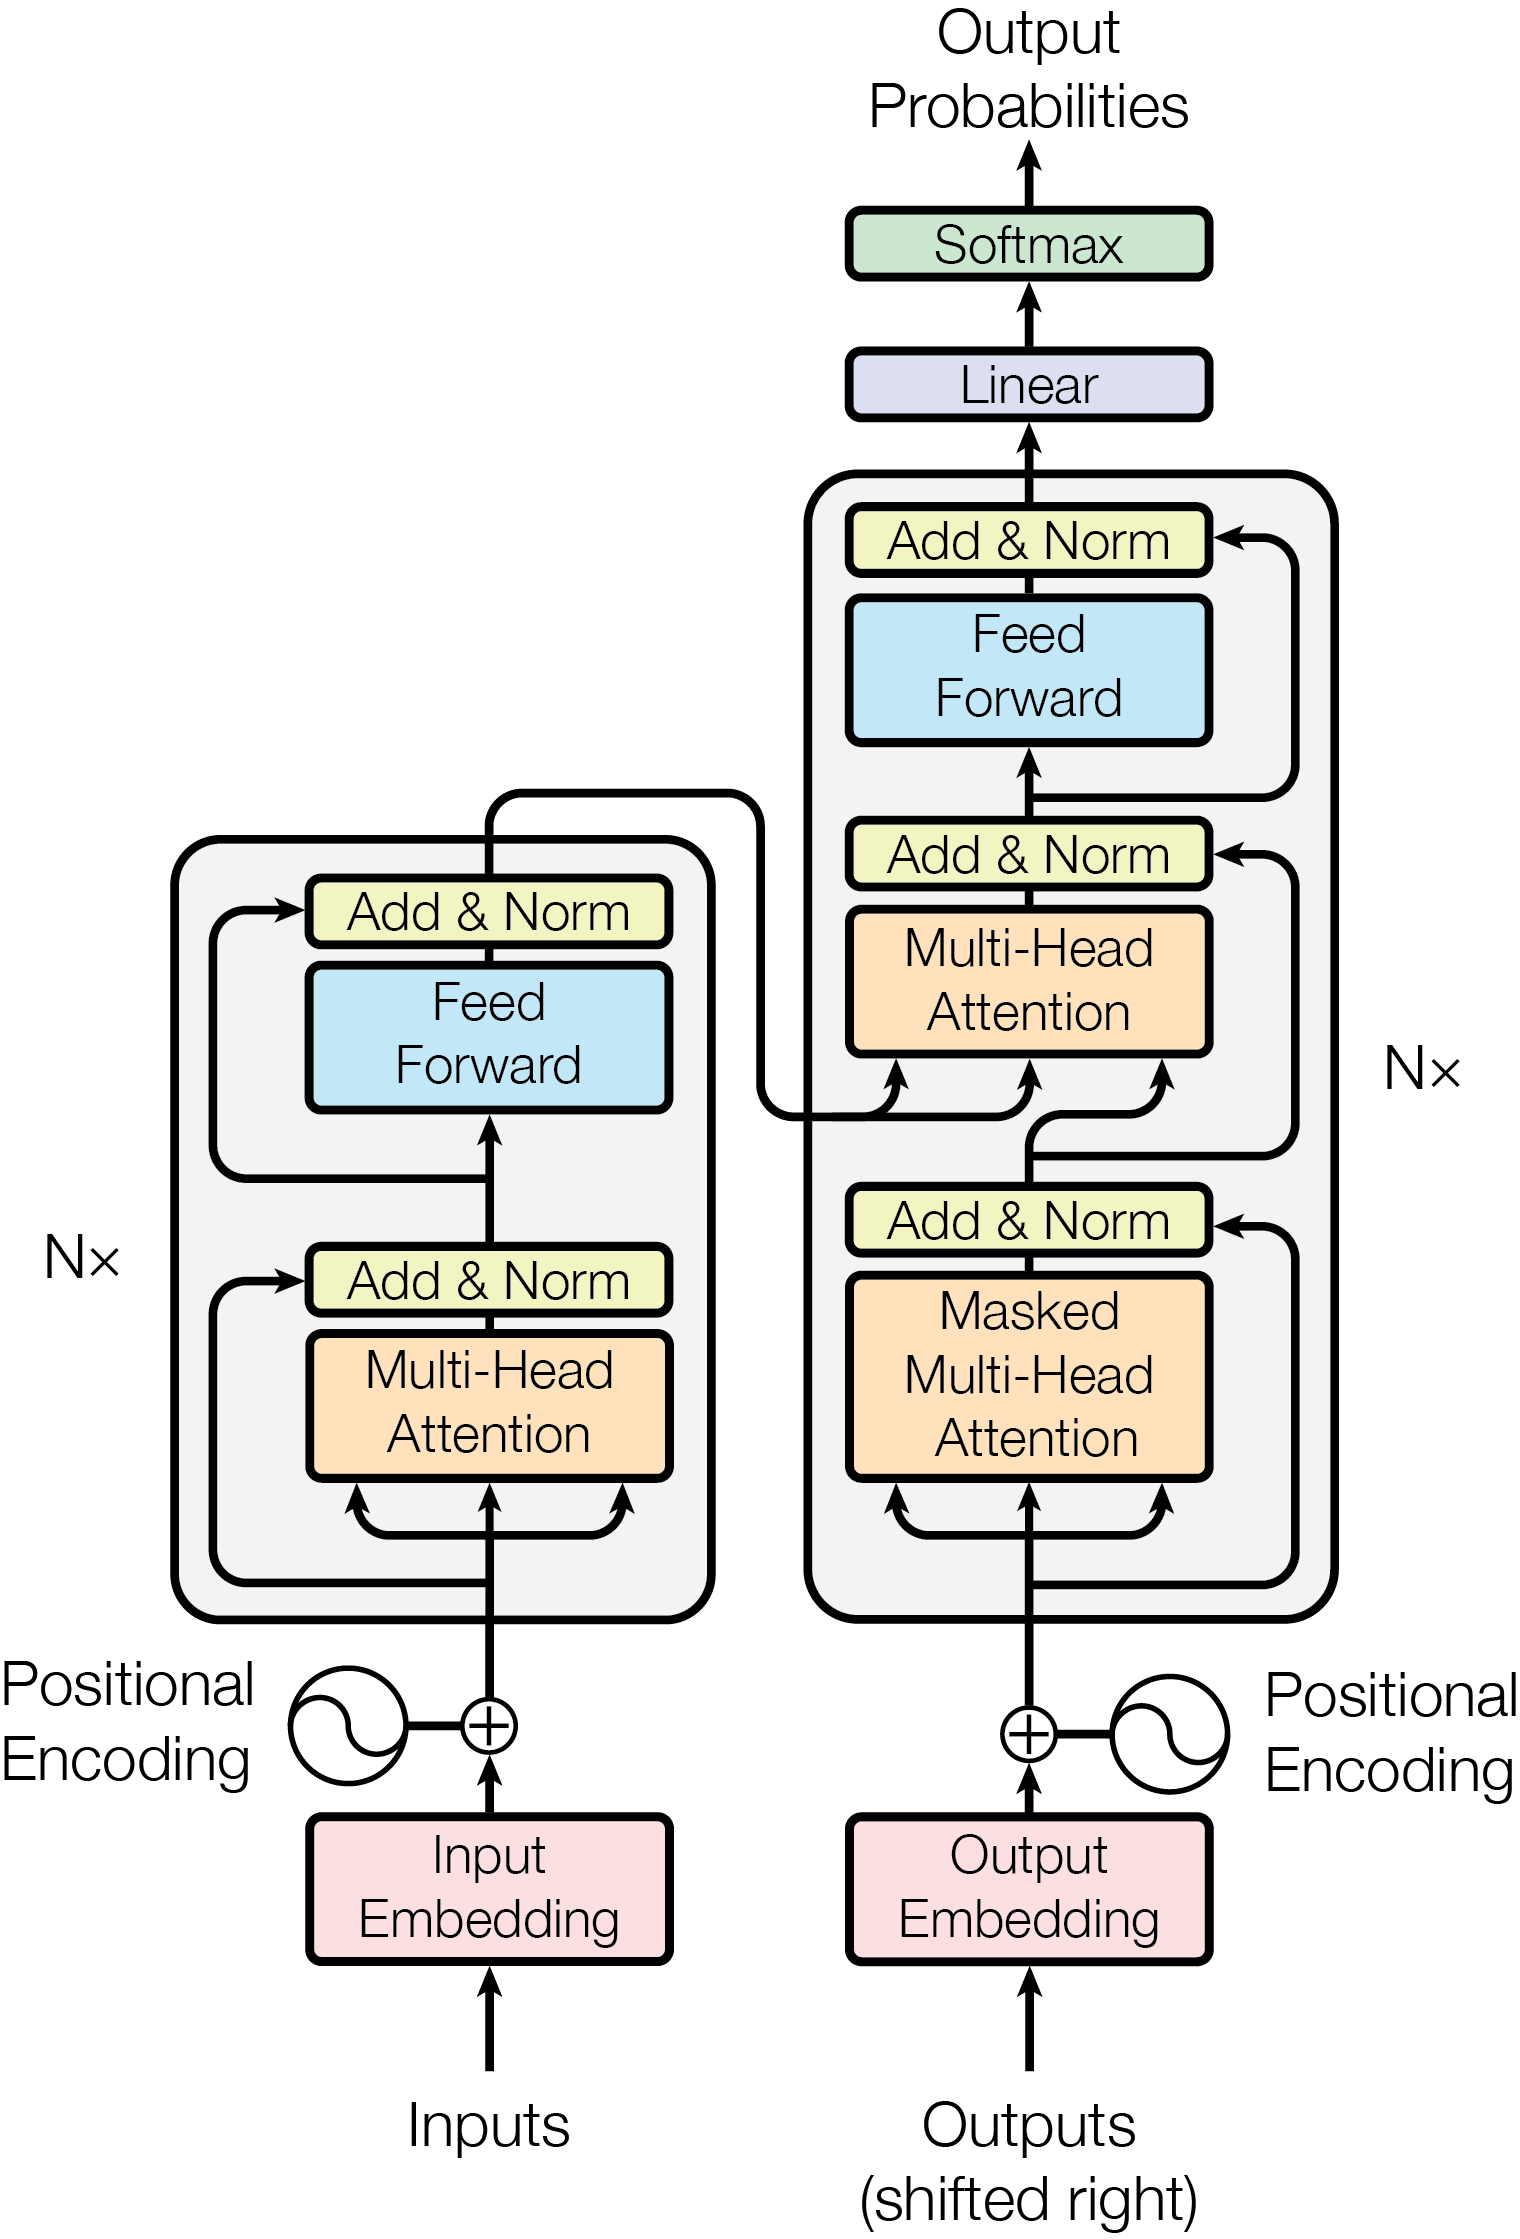
\includegraphics[scale=0.20]{figs/architecture.png}
	\caption{Schemat blokowy architektury transformera}
	\label{fig:transformer_architecture}
\end{figure}

\bibliographystyle{unsrt}
\bibliography{refs}

\end{document}

% \chapter{Wprowadzenie}\label{ch:intro}


% \section{Motywacja}\label{sec:motiv}

% Sed ut perspiciatis, unde omnis iste natus error sit voluptatem accusantium doloremque laudantium, totam rem aperiam eaque ipsa, quae ab illo inventore veritatis et quasi architecto beatae vitae dicta sunt, explicabo. 
% Nemo enim ipsam voluptatem, quia voluptas sit, aspernatur aut odit aut fugit, sed quia consequuntur magni dolores eos, qui ratione voluptatem sequi nesciunt, neque porro quisquam est, qui dolorem ipsum, quia dolor sit, amet, consectetur, adipisci velit, sed quia non numquam eius modi tempora incidunt, ut labore et dolore magnam aliquam quaerat voluptatem. 
% Ut enim ad minima veniam, quis nostrum exercitationem ullam corporis suscipit laboriosam, nisi ut aliquid ex ea commodi consequatur? 
% Quis autem vel eum iure reprehenderit, qui in ea voluptate velit esse, quam nihil molestiae consequatur, vel illum, qui dolorem eum fugiat, quo voluptas nulla pariatur?

% At vero eos et accusamus et iusto odio dignissimos ducimus, qui blanditiis praesentium voluptatum deleniti atque corrupti, quos dolores et quas molestias excepturi sint, obcaecati cupiditate non provident, similique sunt in culpa, qui officia deserunt mollitia animi, id est laborum et dolorum fuga. 
% Et harum quidem rerum facilis est et expedita distinctio. 
% Nam libero tempore, cum soluta nobis est eligendi optio, cumque nihil impedit, quo minus id, quod maxime placeat, facere possimus, omnis voluptas assumenda est, omnis dolor repellendus. 
% Temporibus autem quibusdam et aut officiis debitis aut rerum necessitatibus saepe eveniet, ut et voluptates repudiandae sint et molestiae non recusandae. 
% Itaque earum rerum hic tenetur a sapiente delectus, ut aut reiciendis voluptatibus maiores alias consequatur aut perferendis doloribus asperiores repellat.


% % \section{Cel i~zakres}\label{sec:aimNscope}

% Celem pracy jest stworzenie aplikacji 

% %%%%%%%%%%%%%%%%%%%%%%%%%%%%%%%%%%%%%%

% \chapter{Tytuł rozdziału}\label{ch:someLabel}


% \section{Typografia}\label{sec:typography}

% Niniejszy dokument powstał w~\href{https://pl.wikipedia.org/wiki/LaTeX}{\LaTeX{u}} --- profesjonalnym, darmowym środowisku do składu tekstu.
% Pisząc tekst o~charakterze naukowym czy inżynierskim, znacznie lepiej jest używać \LaTeX{a} niż Worda~\cite{bookOetiker2022}.
% \LaTeX{a} możesz zainstalować na swoim komputerze lub używać środowisk internetowych, których przykładem jest \href{https://www.overleaf.com}{Overleaf}.


% \section{To i~owo}\label{sec:someLabel}

% Przykładowe równanie to
% \begin{equation}
%     E = m c^2
%     \label{eq:Emc2},
% \end{equation}
% gdzie $E$ oznacza \dots\ 

% Opis równania w~pliku {\tt .tex} powinien następować tuż pod równaniem, bez pustej linii między równaniem a~opisem, ponieważ pusta linia w~pliku {\tt .tex}  skutkuje nowym akapitem w~pliku {\tt .pdf}.

% Nowy akapit jest wcięty.
% Jeśli z~jakiegoś szczególnego powodu nie chcesz, aby nowy akapit był wcięty, użyj komendy \verb!\noindent! na początku tego akapitu.

% Równanie~\eqref{eq:Emc2} wygląda znajomo.
% Zauważ wygodne linkowanie z~tekstu do równania.
% Osiąga się to łatwo, stosując dedykowaną etykietę, jak możesz sprawdzić w~źródłowym pliku {\tt .tex}.
% Podobnie można (i~należy) linkować rysunki (patrz  Rys.~\ref{fig:formats}), tabele (Tab.~\ref{tab:err}), sekcje (np.\ Sekcja~\ref{sec:aimNscope}) i~rozdziały (np.\ Rozdz.~\ref{ch:disco}).
% A~to jest zdanie cytujące książkę~\cite{bookSurname2020} i~artykuł~\cite{artSurname2022}.


% \section{Rysunki}\label{sec:figs}

% Rysunki, które nie są zdjęciami, powinny być \href{https://pl.wikipedia.org/wiki/Grafika_wektorowa}{\em grafikami wektorowymi}.
% Jest to szczególnie ważne w~przypadku wykresów (jak na Rys.~\ref{fig:formats}) i~schematów blokowych (jak na Rys.~\ref{fig:xhy}). 
% Odpowiednimi formatami tego rodzaju grafik obsługiwanymi w~\LaTeX{u} są \href{https://pl.wikipedia.org/wiki/Encapsulated_PostScript}{Encapsulated PostScript} (EPS) and \href{https://pl.wikipedia.org/wiki/Portable_Document_Format}{Portable Document Format} (PDF).

% \begin{figure}
% 	\centering
% 	\begin{subfigure}[b]{\columnwidth}
% 	\centering
% 	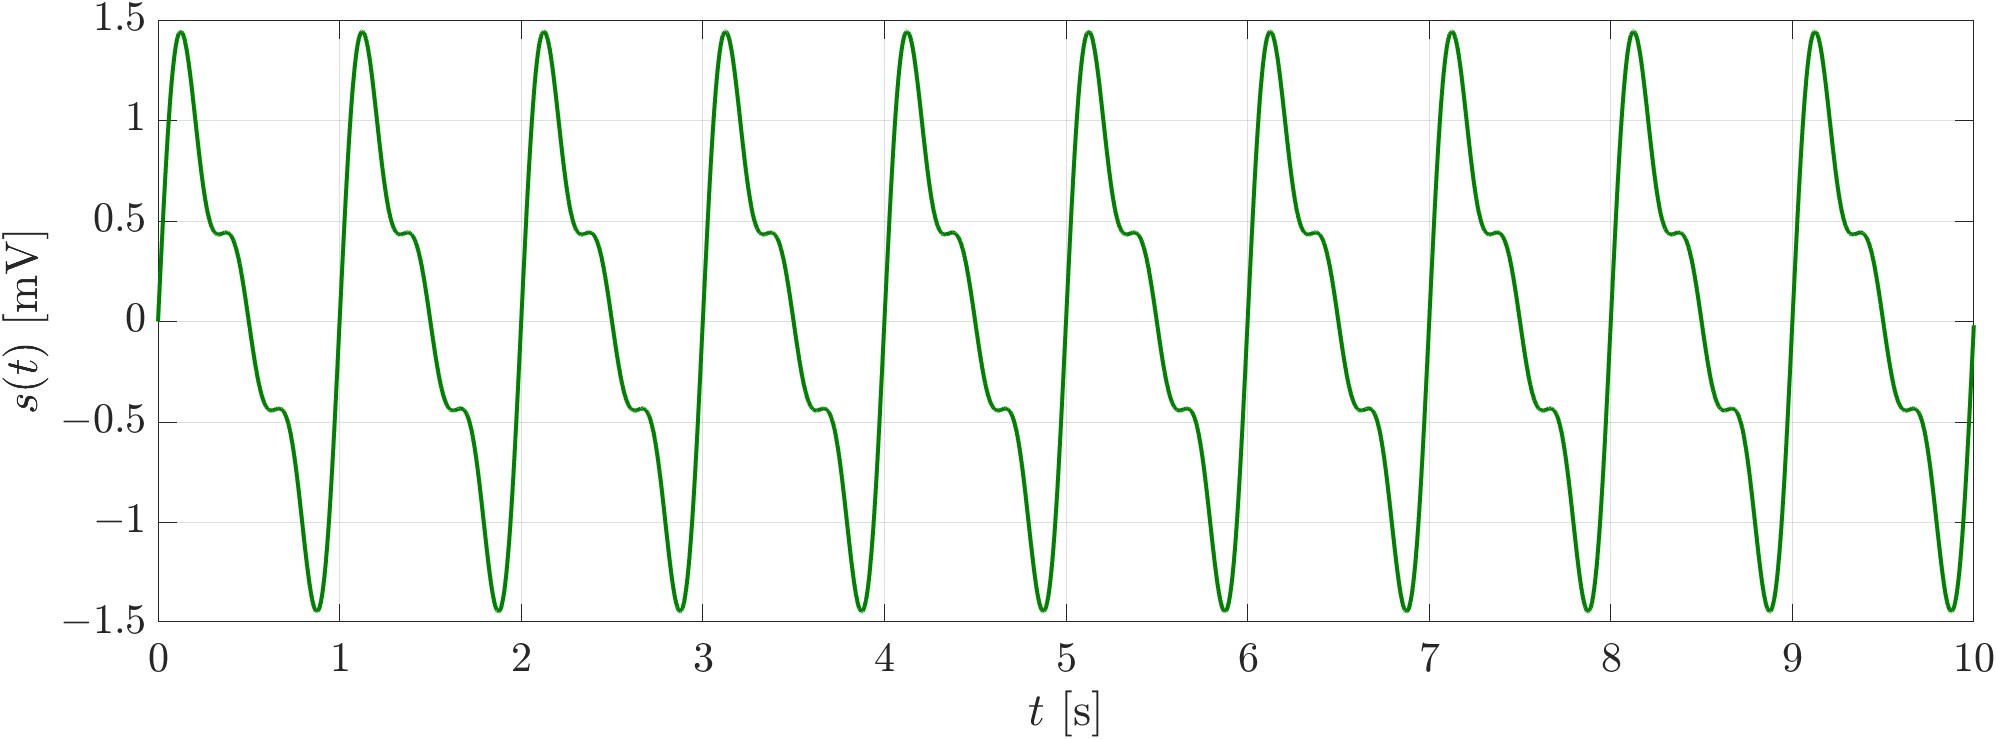
\includegraphics[width=\columnwidth]{figs/someSignal.jpg}
% 	\caption{Brzydki, skompresowany JPG.
%     Powiększ go na ekranie, aby zobaczyć artefakty kompresji.}
% 	\label{fig:jpg}
% 	\end{subfigure}
	
% 	\vspace{6mm}
	
% 	\begin{subfigure}[b]{\columnwidth}
% 	\centering
% 	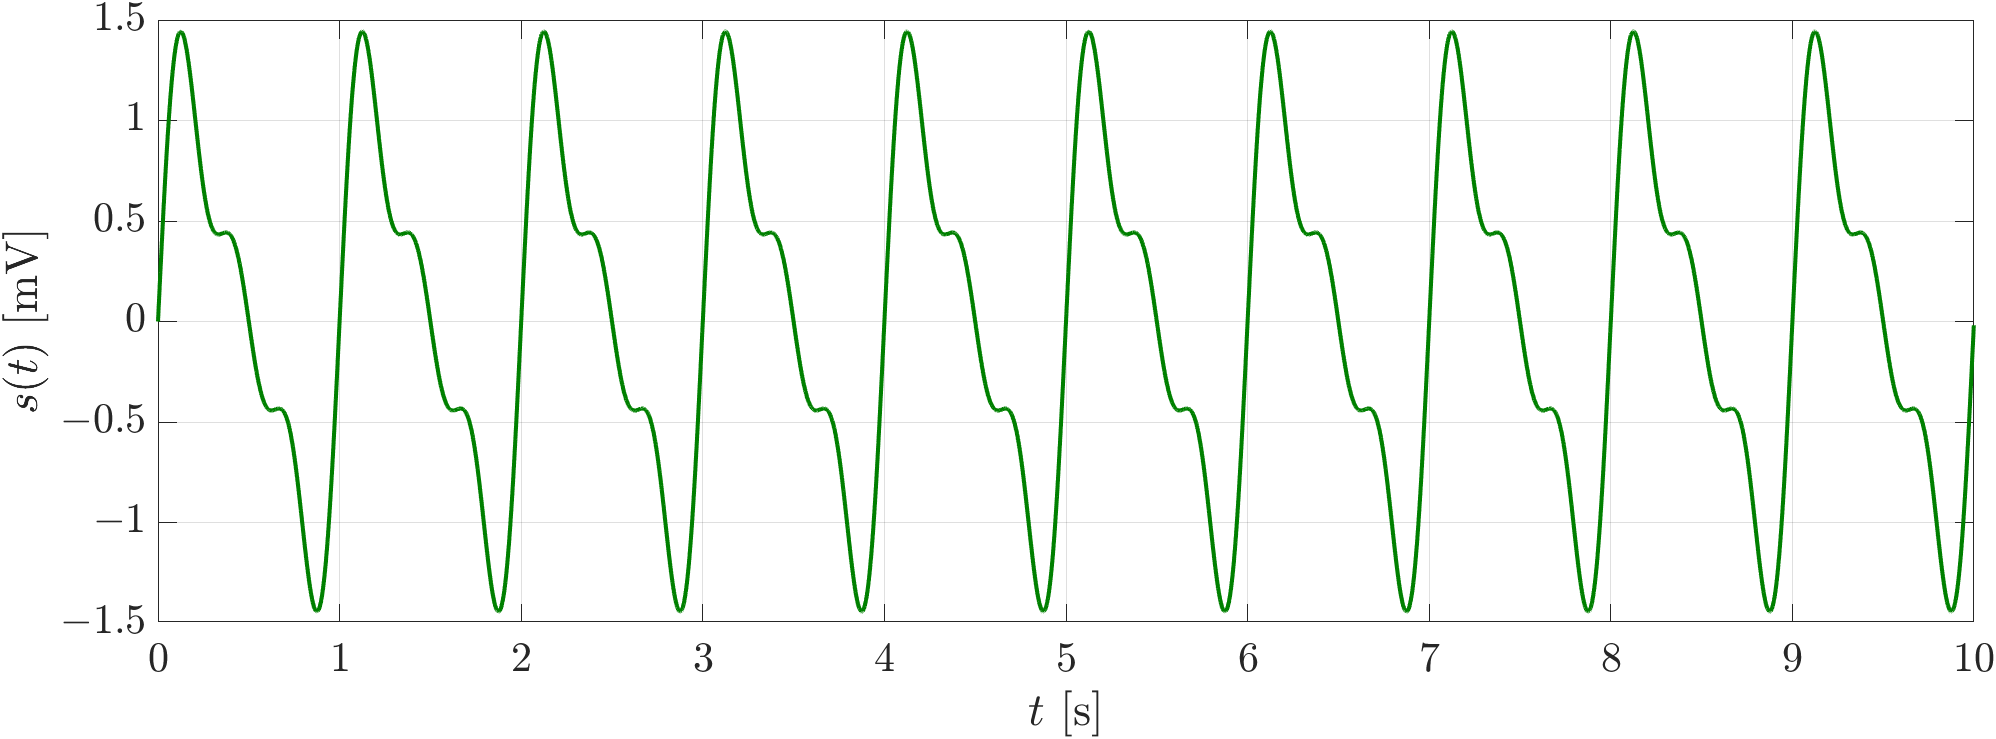
\includegraphics[width=\columnwidth]{figs/someSignal.png}
% 	\caption{Nieco ładniejszy PNG, lecz nadal jest to \href{https://pl.wikipedia.org/wiki/Grafika_rastrowa}{grafika rastrowa}.}
% 	\label{fig:png}
% 	\end{subfigure}
	
% 	\vspace{6mm}
	
% 	\begin{subfigure}[b]{\columnwidth}
% 	\centering
% 	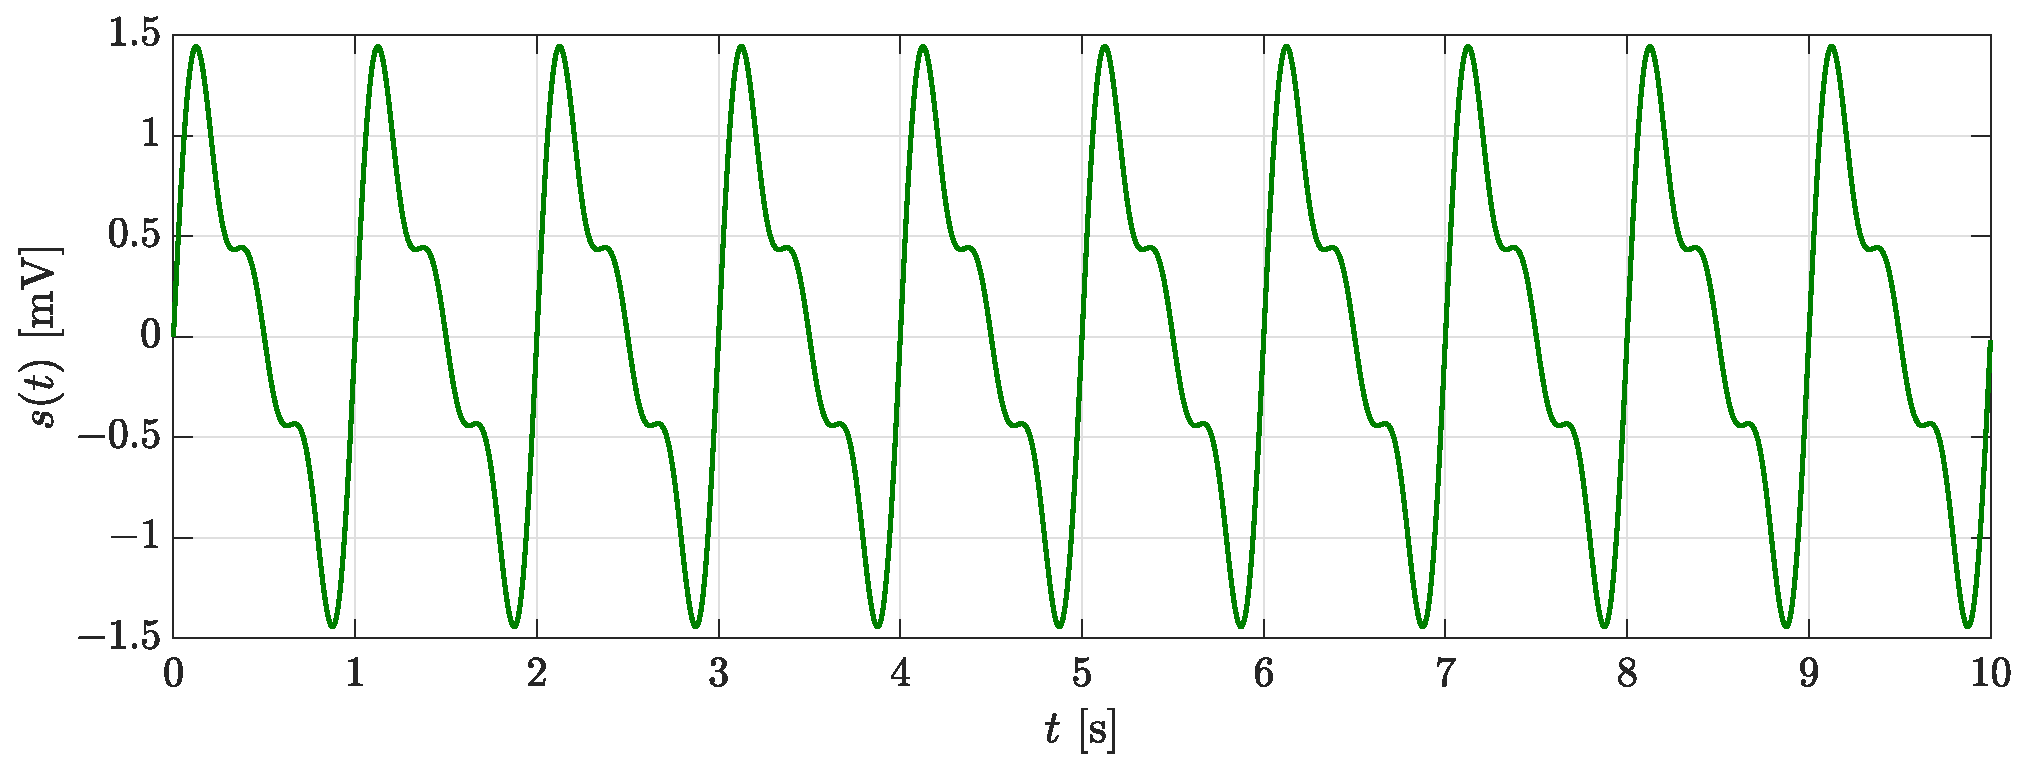
\includegraphics[width=\columnwidth]{figs/someSignal.eps}
% 	\caption{Ładny, \href{https://pl.wikipedia.org/wiki/Grafika_wektorowa}{wektorowy} EPS.
%     Może być powiększany na ekranie celem dokładniejszego oglądu.}
% 	\label{fig:eps}
% 	\end{subfigure}
 
% 	\caption[Krótki podpis na potrzeby {\em Spisu rysunków}]
%     {Różnice w~jakości grafik zależnie od formatu. 
% 	Pamiętaj o~poprawnym opisie osi i~podaniu jednostek fizycznych.
% 	Aby wykres był czytelny, zadbaj o~odpowiednio dużą wielkość czcionki etykiet.}
% 	\label{fig:formats}
% \end{figure}

% \subsection{Schematy blokowe}\label{ssec:flow}

% Wygodnym i~darmowym narzędziem do tworzenia schematów blokowych jest \href{https://draw.io}{draw.io}.
% Umożliwia eksport do grafik wektorowych: {\tt File | Export as | PDF}.\footnote{Nie zapomnij zaznaczyć opcji {\tt Crop}, aby uniknąć niepotrzebnych białych marginesów.}
% Po wybraniu {\tt Extras | Mathematical Typesetting} można łatwo dodawać \href{https://www.diagrams.net/doc/faq/math-typesetting}{wyrażenia matematyczne}. 
% Rysunek~\ref{fig:xhy} przedstawia przykładowy schemat blokowy utworzony w~\href{https://draw.io}{draw.io}.

% \begin{figure}
%     \centering
%     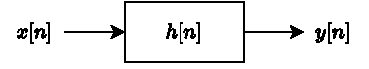
\includegraphics[width=0.5\textwidth]{figs/xhy.pdf}
%     \caption[Filtr]
%     {
%     Przykładowy schemat blokowy utworzony w~\href{https://draw.io}{draw.io}.
%     Zauważ, że jest to  \href{https://pl.wikipedia.org/wiki/Grafika_wektorowa}{grafika wektorowa}.
%     Schematy blokowe {\em nigdy} nie powinny być  \href{https://pl.wikipedia.org/wiki/Grafika_rastrowa}{grafikami rastrowymi}.
%     Podpis powinien informować, co schemat blokowy przedstawia.
%     W~tym przypadku sygnał $x[n]$ przetwarzany jest przez filtr $h[n]$, który na wyjściu daje sygnał $y[n]$.
%     }
%     \label{fig:xhy}
% \end{figure}

% \subsection{Umiejscowienie rysunków i~tabel}\label{ssec:place}

% Nierzadko może się wydawać, że \LaTeX{} umieszcza rysunki i~tabele w~niewłaściwych miejscach.
% Nie martw się --- w 99,(9)\% przypadków \LaTeX{} ma rację i~naprawdę wie lepiej.
% Zauważ, że w~każdej profesjonalnie wydanej książce rysunki oraz tabele umieszczone są na górze albo na dole strony (albo na osobnej stronie, jeśli rysunek czy tabela są odpowiednio duże), nie pomiędzy fragmentami tekstu.
% Tak robi to również \LaTeX{}, gdyż właśnie tak należy to robić.
% Zapomnij o~swoich starych nawykach w~tym względzie.
% Jeżeli naprawdę musisz umieścić rysunek czy tabelę w~jakimś szczególnym miejscu, jest na to prosty sposób~\cite{bookOetiker2022}.


% \section{Tabele}\label{sec:tab}

% Proste tabele tworzy się w~\LaTeX{u} bardzo łatwo.
% Kiedy potrzeba bardziej skomplikowanego układu, pomocny może okazać się generator dostępny pod adresem \url{https://www.tablesgenerator.com/latex_tables}.

% W~przeciwieństwie do rysunków tabele zwykle posiadają podpis nad, nie pod nimi.


% \section{Fragmenty kodu}\label{sec:code}

% Jeśli potrzebujesz przedstawić fragment kodu Twojego programu komputerowego, umieść go w~otoczeniu \verb!verbatim!.
% W~efekcie będzie on złożony jak w~typowym środowisku programistycznym, tj.\ \href{https://en.wikipedia.org/wiki/Monospaced_font}{\em czcionką o~jednakowej szerokości znaków}. 
% Poniżej przedstawiono fragment kodu w~języku MATLAB, generujący Rys.~\ref{fig:eps}.
% Przypomnijmy, że dobrą praktyką jest komentowanie kodu.

% \begin{verbatim}
% set(groot, 'DefaultAxesTickLabelInterpreter', 'LaTeX');  
% set(groot, 'DefaultLegendInterpreter'       , 'LaTeX');
% set(groot, 'DefaultTextInterpreter'         , 'LaTeX');
% set(0    , 'DefaultFigureColor'             , 'w'    );

% fs = 1e3;  % Sampling frequency [Hz].
% t  = 0 : 1/fs : 10 - 1/fs;  % Discrete time domain [s].
% f  = 1 : 3;  % Some frequencies [Hz].

% s = zeros(size(t));
% for ii = 1 : length(f)
%     s = s + sin(2 * pi * f(ii) * t) / ii;
% end

% figure('Position', [1e2 1e2 15e2 5e2])
% plot(t, s, 'Color', [0 .5 0], 'LineWidth', 2);  grid
% xtickformat('$%g$');  ytickformat('$%g$')  % For proper minuses.
% set(gca, 'FontSize', 20)
% xlabel('$t$ [s]');  ylabel('$s(t)$ [mV]')

% set(gcf, 'renderer', 'painters')  % For vector-graphics output.
% exportgraphics(gcf, 'someSignal.eps')
% \end{verbatim}

% Taki kod jest oczywiście zbyt trywialny, aby przedstawiać go w~pracy; służy tu jedynie jako ilustrujący przykład.


% \section{Typowe błędy}\label{sec:mist}

% Typowe błędy formatowania oraz sposoby na ich uniknięcie przedstawia Tab.~\ref{tab:err} zaczerpnięta z~opracowania~\cite{miscSieluzycki2024}, które warto przeczytać.

% Rozróżniaj między \href{https://pl.wikipedia.org/wiki/Dywiz}{łącznikiem} (\dywiz{}), \href{https://pl.wikipedia.org/wiki/Pauza_i_p%C3%B3%C5%82pauza}{półpauzą} (--), \href{https://pl.wikipedia.org/wiki/Pauza_i_p%C3%B3%C5%82pauza}{pauzą} \mbox{(---)} oraz~\href{https://pl.wikipedia.org/wiki/Plus_i_minus}{znakiem minus} ($-$).
% Użycie łącznika w~roli \href{https://pl.wikipedia.org/wiki/My%C5%9Blnik}{myślnika} jest rażącym błędem.
% Znak minus wymaga użycia {\em trybu matematycznego};
% przykładowo, \verb!$-1$! w~pliku {\tt .tex} skutkuje $-1$ w~pliku {\tt .pdf}.
% Przypomnijmy także, że --- w przeciwieństwie do języków programowania --- w~matematyce gwiazdka (*) nie oznacza zwykłego mnożenia, ale \href{https://pl.wikipedia.org/wiki/Splot_(analiza_matematyczna)}{splot}.
% Dlatego nie należy jej używać do oznaczenia zwykłego mnożenia w~wyrażeniach matematycznych.
% Kiedy w~otoczeniu matematycznym używasz przecinka jako separatora części całkowitej i~reszty liczby (a~tak właśnie, czyli z~przecinkiem zamiast kropki, pisze się w~dokumentach polskojęzycznych), pamiętaj, aby przecinek otoczyć klamrami, np.\ \verb!$2{,}3$!; w~przeciwnym razie za przecinkiem pojawi się niechciany odstęp~\cite{miscSieluzycki2024}. 

% Dobrym zwyczajem w~języku polskim jest niepozostawianie wyrazów jednoliterowych na końcu wiersza.\footnote{Zasada ta nie dotyczy języka angielskiego.}
% Aby to osiągnąć, wyraz jednoliterowy należy połączyć z~wyrazem następującym niełamliwą spacją, która w~pliku {\tt .tex} ma postać tyldy; np.\ \verb!w~porządku!.

% W~przeciwieństwie do języka angielskiego w~języku polskim \href{https://sjp.pwn.pl/zasady/Podzial-wyrazu-w-miejscu-lacznika;629553.html}{złamanie wiersza w~miejscu łącznika} oznacza potrzebę przeniesienia łącznika do nowego wiersza.
% Dotyczy to konstrukcji w~rodzaju {\em czerwono\dywiz{}czarny}\footnote{Ale nie {\em ciemnoczerwony}, gdzie łącznika być nie powinno.}, {\em jesienno\dywiz{}zimowy}, {\em badawczo\dywiz{}rozwojowy}, {\em matematyczno\dywiz{}techniczny}.
% Aby poprawna obsługa takich konstrukcji zachodziła automatycznie, łącznik (zwany także dywizem) zapisuj w~pliku {\tt .tex} {\em explicite}, tj.\ np.\ \verb!słodko\dywiz{}gorzki!.
% Pakiet {\tt polski}, wykorzystany w~niniejszym szablonie, zadba o~resztę.

% \begin{table}
% \centering
% \caption[Typowe błędy formatowania]
% {Typowe błędy formatowania. 
% {\em Ryzyko} oznacza tu dwie sytuacje: 1)~wartość liczbowa na końcu wiersza, zaś jednostka fizyczna w~kolejnym wierszu, co jest oczywiście niewłaściwe; 2)~łącznik na końcu wiersza, co w~języku polskim jest niepoprawne.
% Źródło:~\cite{miscSieluzycki2024}.}
% \begin{tabular}{ll||ll}
% \multicolumn{2}{l||}{\bf Źle}         & \multicolumn{2}{l}{\bf Dobrze}       \\ \hline
% \multicolumn{1}{l|}{Zapis w~{\tt .tex}} & Efekt w~{\tt .pdf} & \multicolumn{1}{l|}{Zapis w~{\tt .tex}} & Efekt w~{\tt .pdf} \\ \hline
% \multicolumn{1}{l|}{\tt 20mV}    & 20mV    & \multicolumn{1}{l|}{\tt 20\~{}mV}    & 20~mV    \\
% \multicolumn{1}{l|}{\tt \$20mV\$}    & $20mV$    & \multicolumn{1}{l|}{\tt \$20\~{}\{\textbackslash{}rm mV\}\$}    & $20~{\rm mV}$    \\
% \multicolumn{1}{l|}{\tt 20 mV}    & Ryzyko   & \multicolumn{1}{l|}{\tt 20\~{}mV}    & 20~mV    \\
% \multicolumn{1}{l|}{\tt \$2 * x\$}    & $2 * x$    & \multicolumn{1}{l|}{\tt \$2 x\$}    & $2 x$    \\
% \multicolumn{1}{l|}{\tt \$2 * 3\$}    & $2 * 3$    & \multicolumn{1}{l|}{\tt \$2 \textbackslash{}cdot 3\$}    & $2 \cdot 3$    \\
% \multicolumn{1}{l|}{\tt MxN}    & MxN    & \multicolumn{1}{l|}{\tt \$M \textbackslash{}times N\$}    & $M \times N$    \\
% \multicolumn{1}{l|}{\tt -1}    & -1    & \multicolumn{1}{l|}{\tt \$-1\$}    & $-1$    \\
% \multicolumn{1}{l|}{\tt \$sin(x)\$}    & $sin(x)$    & \multicolumn{1}{l|}{\tt \$\textbackslash{}sin(x)\$}    & $\sin(x)$    \\
% \multicolumn{1}{l|}{\tt \$max(x)\$}    & $max(x)$    & \multicolumn{1}{l|}{\tt \$\textbackslash{}max(x)\$}    & $\max(x)$    \\
% \multicolumn{1}{l|}{\tt \$s\_\{out\}\$}    & $s_{out}$    & \multicolumn{1}{l|}{\tt \$s\_\{\textbackslash{}rm out\}\$}    & $s_{\rm out}$    \\
% \multicolumn{1}{l|}{\tt \$u\_\{\textbackslash{}rm ij\}\$\ }    & $u_{\rm ij}$    & \multicolumn{1}{l|}{\tt \$u\_\{ij\}\$}    & $u_{ij}$    \\
% \multicolumn{1}{l|}{\tt \$\{\textbackslash{}bf U\}\^{}T\$}    & ${\bf U}^T$    & \multicolumn{1}{l|}{\tt \$\{\textbackslash{}bf U\}\^{}\{\textbackslash{}rm T\}\$}    & ${\bf U}^{\rm T}$ \\ 
% \multicolumn{1}{l|}{\tt "cytat"}    & "cytat"    & \multicolumn{1}{l|}{\tt ,,cytat''}    & ,,cytat'' \\
% \multicolumn{1}{l|}{\tt biało-żółty}    & Ryzyko  & \multicolumn{1}{l|}{\tt biało\textbackslash{}dywiz\{\}żółty}    & biało\dywiz{}żółty 
% \end{tabular}
% \label{tab:err}
% \end{table}


% \section{Odniesienia do źródeł informacji}\label{sec:sources}

% Za wszelką cenę unikaj popełnienia \href{https://pl.wikipedia.org/wiki/Plagiat}{plagiatu}.
% Pamiętaj o~poprawnym cytowaniu materiałów źródłowych, również w~podpisach rysunków i~tabel.

% W~{\em Bibliografii} na końcu pracy zawrzyj tylko te pozycje, które cytujesz w~tekście pracy.
% Oznacza to, że każdą z~pozycji podanych w~{\em Bibliografii} należy zacytować.
% W~\LaTeX{u} jest to łatwe --- patrz \href{https://pl.wikipedia.org/wiki/BibTeX}{BibTeX}, który sformatuje wszystkie pozycje wg stylu, który określa się komendą \verb!\bibliographystyle! w~pliku {\tt .tex}.

% %%%%%%%%%%%%%%%%%%%%%%%%%%%%%%%%%%%%%%

% \chapter{Dyskusja}\label{ch:disco}

% Dobrze napisana praca dyplomowa powinna zawierać dobrze napisaną dyskusję, z~odniesieniami do istniejącej literatury oraz do celu pracy.

% %%%%%%%%%%%%%%%%%%%%%%%%%%%%%%%%%%%%%%

% \bibliographystyle{plain}
% \bibliography{refs}

% \appendix

% \hypersetup{linkcolor=black}
% \listoffigures

% \hypersetup{linkcolor=black}
% \listoftables
